\documentclass{standalone}
\usepackage{tikz}
\usetikzlibrary{patterns, positioning}


\begin{document}
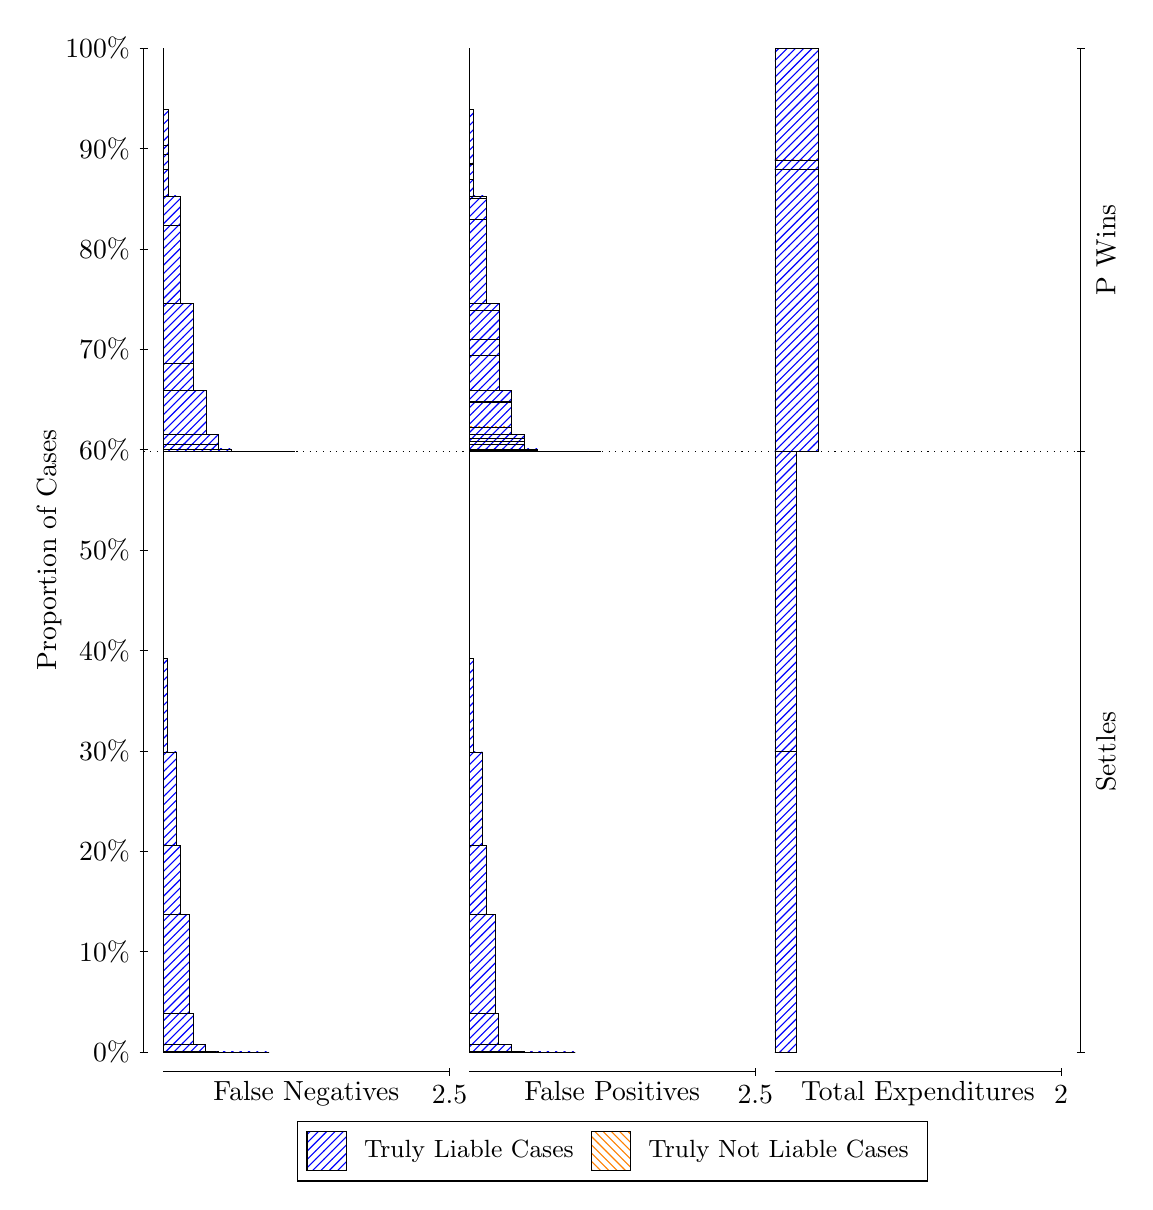
\begin{tikzpicture}
\draw[black, very thin] (1.5,1.75) -- (1.5,14.5);
\node[rotate=90, text=black, anchor=center] at (0.3, 8.125) {Proportion of Cases};
\draw[black, very thin] (1.45,1.75) -- (1.55,1.75);
\node[text=black, anchor=east] at (1.45, 1.75) {0\%};
\draw[black, very thin] (1.45,3.025) -- (1.55,3.025);
\node[text=black, anchor=east] at (1.45, 3.025) {10\%};
\draw[black, very thin] (1.45,4.3) -- (1.55,4.3);
\node[text=black, anchor=east] at (1.45, 4.3) {20\%};
\draw[black, very thin] (1.45,5.575) -- (1.55,5.575);
\node[text=black, anchor=east] at (1.45, 5.575) {30\%};
\draw[black, very thin] (1.45,6.85) -- (1.55,6.85);
\node[text=black, anchor=east] at (1.45, 6.85) {40\%};
\draw[black, very thin] (1.45,8.125) -- (1.55,8.125);
\node[text=black, anchor=east] at (1.45, 8.125) {50\%};
\draw[black, very thin] (1.45,9.4) -- (1.55,9.4);
\node[text=black, anchor=east] at (1.45, 9.4) {60\%};
\draw[black, very thin] (1.45,10.675) -- (1.55,10.675);
\node[text=black, anchor=east] at (1.45, 10.675) {70\%};
\draw[black, very thin] (1.45,11.95) -- (1.55,11.95);
\node[text=black, anchor=east] at (1.45, 11.95) {80\%};
\draw[black, very thin] (1.45,13.225) -- (1.55,13.225);
\node[text=black, anchor=east] at (1.45, 13.225) {90\%};
\draw[black, very thin] (1.45,14.5) -- (1.55,14.5);
\node[text=black, anchor=east] at (1.45, 14.5) {100\%};

\draw[black, very thin] (13.4,1.75) -- (13.4,14.5);
\draw[black, very thin] (13.35,1.75) -- (13.45,1.75);
\node[anchor=west] at (13.35, 1.75) {};
\draw[black, very thin] (13.35,9.3748) -- (13.45,9.3748);
\node[anchor=west] at (13.35, 9.3748) {};
\draw[black, very thin] (13.35,14.5) -- (13.45,14.5);
\node[anchor=west] at (13.35, 14.5) {};

\draw[black, very thin, pattern color=blue, pattern=north east lines] (1.75,1.75) rectangle (3.0943,1.75);
\draw[black, very thin, pattern color=blue, pattern=north east lines] (1.75,1.75) rectangle (2.9329,1.75);
\draw[black, very thin, pattern color=blue, pattern=north east lines] (1.75,1.75) rectangle (2.7714,1.75);
\draw[black, very thin, pattern color=blue, pattern=north east lines] (1.75,1.75) rectangle (2.6099,1.7502);
\draw[black, very thin, pattern color=blue, pattern=north east lines] (1.75,1.7502) rectangle (2.5857,1.7502);
\draw[black, very thin, pattern color=blue, pattern=north east lines] (1.75,1.7502) rectangle (2.4484,1.7576);
\draw[black, very thin, pattern color=blue, pattern=north east lines] (1.75,1.7576) rectangle (2.4242,1.7576);
\draw[black, very thin, pattern color=blue, pattern=north east lines] (1.75,1.7576) rectangle (2.2869,1.8422);
\draw[black, very thin, pattern color=blue, pattern=north east lines] (1.75,1.8422) rectangle (2.2627,1.8422);
\draw[black, very thin, pattern color=blue, pattern=north east lines] (1.75,1.8422) rectangle (2.1254,2.2353);
\draw[black, very thin, pattern color=blue, pattern=north east lines] (1.75,2.2353) rectangle (2.1012,2.2354);
\draw[black, very thin, pattern color=blue, pattern=north east lines] (1.75,2.2354) rectangle (2.077,3.499);
\draw[black, very thin, pattern color=blue, pattern=north east lines] (1.75,3.499) rectangle (1.964,4.3781);
\draw[black, very thin, pattern color=blue, pattern=north east lines] (1.75,4.3781) rectangle (1.9397,4.3787);
\draw[black, very thin, pattern color=blue, pattern=north east lines] (1.75,4.3787) rectangle (1.9155,5.5624);
\draw[black, very thin, pattern color=blue, pattern=north east lines] (1.75,5.5624) rectangle (1.8025,6.7462);
\draw[black, very thin, pattern color=blue, pattern=north east lines] (1.75,6.7462) rectangle (1.7783,6.7467);
\draw[black, very thin, pattern color=blue, pattern=north east lines] (1.75,6.7467) rectangle (1.754,7.6258);
\draw[black, very thin, pattern color=orange, pattern=north west lines] (1.75,7.6258) rectangle (1.75,7.6258);
\draw[black, very thin, pattern color=blue, pattern=north east lines] (1.75,7.6258) rectangle (1.75,9.3748);
\draw[black, very thin, pattern color=blue, pattern=north east lines] (1.75,9.3748) rectangle (3.4213,9.3748);
\draw[black, very thin, pattern color=blue, pattern=north east lines] (1.75,9.3748) rectangle (3.2599,9.3748);
\draw[black, very thin, pattern color=blue, pattern=north east lines] (1.75,9.3748) rectangle (3.2599,9.3748);
\draw[black, very thin, pattern color=blue, pattern=north east lines] (1.75,9.3748) rectangle (3.0984,9.3748);
\draw[black, very thin, pattern color=blue, pattern=north east lines] (1.75,9.3748) rectangle (3.0984,9.3748);
\draw[black, very thin, pattern color=blue, pattern=north east lines] (1.75,9.3748) rectangle (2.9369,9.375);
\draw[black, very thin, pattern color=blue, pattern=north east lines] (1.75,9.375) rectangle (2.7754,9.377);
\draw[black, very thin, pattern color=blue, pattern=north east lines] (1.75,9.377) rectangle (2.7754,9.3782);
\draw[black, very thin, pattern color=blue, pattern=north east lines] (1.75,9.3782) rectangle (2.6139,9.4104);
\draw[black, very thin, pattern color=blue, pattern=north east lines] (1.75,9.4104) rectangle (2.4524,9.4718);
\draw[black, very thin, pattern color=blue, pattern=north east lines] (1.75,9.4718) rectangle (2.4524,9.5885);
\draw[black, very thin, pattern color=blue, pattern=north east lines] (1.75,9.5885) rectangle (2.291,10.155);
\draw[black, very thin, pattern color=blue, pattern=north east lines] (1.75,10.155) rectangle (2.1295,10.496);
\draw[black, very thin, pattern color=blue, pattern=north east lines] (1.75,10.496) rectangle (2.1295,11.254);
\draw[black, very thin, pattern color=blue, pattern=north east lines] (1.75,11.254) rectangle (1.968,12.247);
\draw[black, very thin, pattern color=blue, pattern=north east lines] (1.75,12.247) rectangle (1.968,12.621);
\draw[black, very thin, pattern color=blue, pattern=north east lines] (1.75,12.621) rectangle (1.8065,12.958);
\draw[black, very thin, pattern color=blue, pattern=north east lines] (1.75,12.958) rectangle (1.8065,13.146);
\draw[black, very thin, pattern color=blue, pattern=north east lines] (1.75,13.146) rectangle (1.8065,13.26);
\draw[black, very thin, pattern color=blue, pattern=north east lines] (1.75,13.26) rectangle (1.8065,13.72);
\draw[black, very thin, pattern color=orange, pattern=north west lines] (1.75,13.72) rectangle (1.75,13.72);
\draw[black, very thin, pattern color=blue, pattern=north east lines] (1.75,13.72) rectangle (1.75,14.5);
\draw[black, very thin, pattern color=orange, pattern=north west lines] (5.6333,1.75) rectangle (6.9777,1.75);
\draw[black, very thin, pattern color=blue, pattern=north east lines] (5.6333,1.75) rectangle (6.9777,1.75);
\draw[black, very thin, pattern color=blue, pattern=north east lines] (5.6333,1.75) rectangle (6.8162,1.75);
\draw[black, very thin, pattern color=blue, pattern=north east lines] (5.6333,1.75) rectangle (6.6547,1.75);
\draw[black, very thin, pattern color=blue, pattern=north east lines] (5.6333,1.75) rectangle (6.4932,1.7502);
\draw[black, very thin, pattern color=orange, pattern=north west lines] (5.6333,1.7502) rectangle (6.469,1.7502);
\draw[black, very thin, pattern color=blue, pattern=north east lines] (5.6333,1.7502) rectangle (6.469,1.7502);
\draw[black, very thin, pattern color=blue, pattern=north east lines] (5.6333,1.7502) rectangle (6.3317,1.7576);
\draw[black, very thin, pattern color=blue, pattern=north east lines] (5.6333,1.7576) rectangle (6.3075,1.7576);
\draw[black, very thin, pattern color=blue, pattern=north east lines] (5.6333,1.7576) rectangle (6.1703,1.8422);
\draw[black, very thin, pattern color=blue, pattern=north east lines] (5.6333,1.8422) rectangle (6.146,1.8422);
\draw[black, very thin, pattern color=blue, pattern=north east lines] (5.6333,1.8422) rectangle (6.0088,2.2353);
\draw[black, very thin, pattern color=blue, pattern=north east lines] (5.6333,2.2353) rectangle (5.9846,2.2354);
\draw[black, very thin, pattern color=orange, pattern=north west lines] (5.6333,2.2354) rectangle (5.9603,2.2354);
\draw[black, very thin, pattern color=blue, pattern=north east lines] (5.6333,2.2354) rectangle (5.9603,3.499);
\draw[black, very thin, pattern color=blue, pattern=north east lines] (5.6333,3.499) rectangle (5.8473,4.3781);
\draw[black, very thin, pattern color=blue, pattern=north east lines] (5.6333,4.3781) rectangle (5.8231,4.3786);
\draw[black, very thin, pattern color=blue, pattern=north east lines] (5.6333,4.3786) rectangle (5.7989,5.5624);
\draw[black, very thin, pattern color=blue, pattern=north east lines] (5.6333,5.5624) rectangle (5.6858,6.7461);
\draw[black, very thin, pattern color=blue, pattern=north east lines] (5.6333,6.7461) rectangle (5.6616,6.7467);
\draw[black, very thin, pattern color=blue, pattern=north east lines] (5.6333,6.7467) rectangle (5.6374,7.6258);
\draw[black, very thin, pattern color=blue, pattern=north east lines] (5.6333,7.6258) rectangle (5.6333,9.3748);
\draw[black, very thin, pattern color=orange, pattern=north west lines] (5.6333,9.3748) rectangle (7.3047,9.3748);
\draw[black, very thin, pattern color=blue, pattern=north east lines] (5.6333,9.3748) rectangle (7.3047,9.3748);
\draw[black, very thin, pattern color=orange, pattern=north west lines] (5.6333,9.3748) rectangle (7.1432,9.3748);
\draw[black, very thin, pattern color=blue, pattern=north east lines] (5.6333,9.3748) rectangle (7.1432,9.3748);
\draw[black, very thin, pattern color=orange, pattern=north west lines] (5.6333,9.3748) rectangle (6.9817,9.3748);
\draw[black, very thin, pattern color=blue, pattern=north east lines] (5.6333,9.3748) rectangle (6.9817,9.3748);
\draw[black, very thin, pattern color=blue, pattern=north east lines] (5.6333,9.3748) rectangle (6.9817,9.3748);
\draw[black, very thin, pattern color=blue, pattern=north east lines] (5.6333,9.3748) rectangle (6.9817,9.3748);
\draw[black, very thin, pattern color=orange, pattern=north west lines] (5.6333,9.3748) rectangle (6.8202,9.3748);
\draw[black, very thin, pattern color=blue, pattern=north east lines] (5.6333,9.3748) rectangle (6.8202,9.3749);
\draw[black, very thin, pattern color=blue, pattern=north east lines] (5.6333,9.3749) rectangle (6.8202,9.375);
\draw[black, very thin, pattern color=orange, pattern=north west lines] (5.6333,9.375) rectangle (6.6587,9.375);
\draw[black, very thin, pattern color=blue, pattern=north east lines] (5.6333,9.375) rectangle (6.6587,9.3755);
\draw[black, very thin, pattern color=blue, pattern=north east lines] (5.6333,9.3755) rectangle (6.6587,9.3782);
\draw[black, very thin, pattern color=blue, pattern=north east lines] (5.6333,9.3782) rectangle (6.4973,9.3866);
\draw[black, very thin, pattern color=orange, pattern=north west lines] (5.6333,9.3866) rectangle (6.4973,9.3866);
\draw[black, very thin, pattern color=blue, pattern=north east lines] (5.6333,9.3866) rectangle (6.4973,9.3903);
\draw[black, very thin, pattern color=blue, pattern=north east lines] (5.6333,9.3903) rectangle (6.4973,9.4104);
\draw[black, very thin, pattern color=blue, pattern=north east lines] (5.6333,9.4104) rectangle (6.3358,9.4711);
\draw[black, very thin, pattern color=blue, pattern=north east lines] (5.6333,9.4711) rectangle (6.3358,9.509);
\draw[black, very thin, pattern color=orange, pattern=north west lines] (5.6333,9.509) rectangle (6.3358,9.509);
\draw[black, very thin, pattern color=blue, pattern=north east lines] (5.6333,9.509) rectangle (6.3358,9.5435);
\draw[black, very thin, pattern color=blue, pattern=north east lines] (5.6333,9.5435) rectangle (6.3358,9.5885);
\draw[black, very thin, pattern color=blue, pattern=north east lines] (5.6333,9.5885) rectangle (6.1743,9.6872);
\draw[black, very thin, pattern color=orange, pattern=north west lines] (5.6333,9.6872) rectangle (6.1743,9.6872);
\draw[black, very thin, pattern color=blue, pattern=north east lines] (5.6333,9.6872) rectangle (6.1743,9.9979);
\draw[black, very thin, pattern color=blue, pattern=north east lines] (5.6333,9.9979) rectangle (6.1743,10.01);
\draw[black, very thin, pattern color=blue, pattern=north east lines] (5.6333,10.01) rectangle (6.1743,10.155);
\draw[black, very thin, pattern color=blue, pattern=north east lines] (5.6333,10.155) rectangle (6.0128,10.592);
\draw[black, very thin, pattern color=blue, pattern=north east lines] (5.6333,10.592) rectangle (6.0128,10.803);
\draw[black, very thin, pattern color=orange, pattern=north west lines] (5.6333,10.803) rectangle (6.0128,10.803);
\draw[black, very thin, pattern color=blue, pattern=north east lines] (5.6333,10.803) rectangle (6.0128,11.166);
\draw[black, very thin, pattern color=blue, pattern=north east lines] (5.6333,11.166) rectangle (6.0128,11.254);
\draw[black, very thin, pattern color=blue, pattern=north east lines] (5.6333,11.254) rectangle (5.8513,12.322);
\draw[black, very thin, pattern color=orange, pattern=north west lines] (5.6333,12.322) rectangle (5.8513,12.322);
\draw[black, very thin, pattern color=blue, pattern=north east lines] (5.6333,12.322) rectangle (5.8513,12.327);
\draw[black, very thin, pattern color=blue, pattern=north east lines] (5.6333,12.327) rectangle (5.8513,12.588);
\draw[black, very thin, pattern color=blue, pattern=north east lines] (5.6333,12.588) rectangle (5.8513,12.621);
\draw[black, very thin, pattern color=blue, pattern=north east lines] (5.6333,12.621) rectangle (5.6899,12.831);
\draw[black, very thin, pattern color=blue, pattern=north east lines] (5.6333,12.831) rectangle (5.6899,13.019);
\draw[black, very thin, pattern color=blue, pattern=north east lines] (5.6333,13.019) rectangle (5.6899,13.042);
\draw[black, very thin, pattern color=blue, pattern=north east lines] (5.6333,13.042) rectangle (5.6899,13.716);
\draw[black, very thin, pattern color=blue, pattern=north east lines] (5.6333,13.716) rectangle (5.6899,13.72);
\draw[black, very thin, pattern color=blue, pattern=north east lines] (5.6333,13.72) rectangle (5.6333,14.5);
\draw[black, very thin, pattern color=orange, pattern=north west lines] (9.5167,1.75) rectangle (9.7892,1.75);
\draw[black, very thin, pattern color=blue, pattern=north east lines] (9.5167,1.75) rectangle (9.7892,5.563);
\draw[black, very thin, pattern color=orange, pattern=north west lines] (9.5167,5.563) rectangle (9.7892,5.563);
\draw[black, very thin, pattern color=blue, pattern=north east lines] (9.5167,5.563) rectangle (9.7892,9.3748);
\draw[black, very thin, pattern color=orange, pattern=north west lines] (9.5167,9.3748) rectangle (10.062,9.3748);
\draw[black, very thin, pattern color=blue, pattern=north east lines] (9.5167,9.3748) rectangle (10.062,12.961);
\draw[black, very thin, pattern color=orange, pattern=north west lines] (9.5167,12.961) rectangle (10.062,12.961);
\draw[black, very thin, pattern color=blue, pattern=north east lines] (9.5167,12.961) rectangle (10.062,13.08);
\draw[black, very thin, pattern color=orange, pattern=north west lines] (9.5167,13.08) rectangle (10.062,13.08);
\draw[black, very thin, pattern color=blue, pattern=north east lines] (9.5167,13.08) rectangle (10.062,14.5);
\draw[black, dotted] (1.5,9.3748) -- (13.4,9.3748);
\draw[black, very thin] (1.75,1.5) -- (5.3833,1.5);
\node[text=black, anchor=north] at (3.5667, 1.5) {False Negatives};
\draw[black, very thin] (5.3833,1.45) -- (5.3833,1.55);
\node[text=black, anchor=north] at (5.3833, 1.45) {2.5};

\draw[black, very thin] (5.6333,1.5) -- (9.2667,1.5);
\node[text=black, anchor=north] at (7.45, 1.5) {False Positives};
\draw[black, very thin] (9.2667,1.45) -- (9.2667,1.55);
\node[text=black, anchor=north] at (9.2667, 1.45) {2.5};

\draw[black, very thin] (9.5167,1.5) -- (13.15,1.5);
\node[text=black, anchor=north] at (11.333, 1.5) {Total Expenditures};
\draw[black, very thin] (13.15,1.45) -- (13.15,1.55);
\node[text=black, anchor=north] at (13.15, 1.45) {2};

\node[text=black, centered, rotate=90] at (13.72, 5.5624) {Settles};
\node[text=black, centered, rotate=90] at (13.72, 11.937) {P Wins};

\draw (7.449999999999999,1.5) node[draw=none] (baseCoordinate) {};
\begin{scope}[align=center]
        \matrix[scale=0.5, draw=black, below=0.5cm of baseCoordinate, nodes={draw}, column sep=0.1cm]{
            \node[rectangle, draw, minimum width=0.5cm, minimum height=0.5cm, pattern color=blue, pattern=north east lines] {}; &
            \node[draw=none, font=\small, text=black] (B) {Truly Liable Cases}; &
            \node[rectangle, draw, minimum width=0.5cm, minimum height=0.5cm, pattern color=orange, pattern=north west lines] {}; &
            \node[draw=none, font=\small, text=black] (B) {Truly Not Liable Cases}; \\
            };
\end{scope}

\end{tikzpicture}
\end{document}